\documentclass[]{article}
\usepackage{lmodern}
\usepackage{amssymb,amsmath}
\usepackage{ifxetex,ifluatex}
\usepackage{fixltx2e} % provides \textsubscript
\ifnum 0\ifxetex 1\fi\ifluatex 1\fi=0 % if pdftex
  \usepackage[T1]{fontenc}
  \usepackage[utf8]{inputenc}
\else % if luatex or xelatex
  \ifxetex
    \usepackage{mathspec}
  \else
    \usepackage{fontspec}
  \fi
  \defaultfontfeatures{Ligatures=TeX,Scale=MatchLowercase}
\fi
% use upquote if available, for straight quotes in verbatim environments
\IfFileExists{upquote.sty}{\usepackage{upquote}}{}
% use microtype if available
\IfFileExists{microtype.sty}{%
\usepackage{microtype}
\UseMicrotypeSet[protrusion]{basicmath} % disable protrusion for tt fonts
}{}
\usepackage[margin=1in]{geometry}
\usepackage{hyperref}
\hypersetup{unicode=true,
            pdftitle={Applied Data Mining Homework 01},
            pdfauthor={Xun Zhao, xz2827},
            pdfborder={0 0 0},
            breaklinks=true}
\urlstyle{same}  % don't use monospace font for urls
\usepackage{color}
\usepackage{fancyvrb}
\newcommand{\VerbBar}{|}
\newcommand{\VERB}{\Verb[commandchars=\\\{\}]}
\DefineVerbatimEnvironment{Highlighting}{Verbatim}{commandchars=\\\{\}}
% Add ',fontsize=\small' for more characters per line
\usepackage{framed}
\definecolor{shadecolor}{RGB}{248,248,248}
\newenvironment{Shaded}{\begin{snugshade}}{\end{snugshade}}
\newcommand{\KeywordTok}[1]{\textcolor[rgb]{0.13,0.29,0.53}{\textbf{#1}}}
\newcommand{\DataTypeTok}[1]{\textcolor[rgb]{0.13,0.29,0.53}{#1}}
\newcommand{\DecValTok}[1]{\textcolor[rgb]{0.00,0.00,0.81}{#1}}
\newcommand{\BaseNTok}[1]{\textcolor[rgb]{0.00,0.00,0.81}{#1}}
\newcommand{\FloatTok}[1]{\textcolor[rgb]{0.00,0.00,0.81}{#1}}
\newcommand{\ConstantTok}[1]{\textcolor[rgb]{0.00,0.00,0.00}{#1}}
\newcommand{\CharTok}[1]{\textcolor[rgb]{0.31,0.60,0.02}{#1}}
\newcommand{\SpecialCharTok}[1]{\textcolor[rgb]{0.00,0.00,0.00}{#1}}
\newcommand{\StringTok}[1]{\textcolor[rgb]{0.31,0.60,0.02}{#1}}
\newcommand{\VerbatimStringTok}[1]{\textcolor[rgb]{0.31,0.60,0.02}{#1}}
\newcommand{\SpecialStringTok}[1]{\textcolor[rgb]{0.31,0.60,0.02}{#1}}
\newcommand{\ImportTok}[1]{#1}
\newcommand{\CommentTok}[1]{\textcolor[rgb]{0.56,0.35,0.01}{\textit{#1}}}
\newcommand{\DocumentationTok}[1]{\textcolor[rgb]{0.56,0.35,0.01}{\textbf{\textit{#1}}}}
\newcommand{\AnnotationTok}[1]{\textcolor[rgb]{0.56,0.35,0.01}{\textbf{\textit{#1}}}}
\newcommand{\CommentVarTok}[1]{\textcolor[rgb]{0.56,0.35,0.01}{\textbf{\textit{#1}}}}
\newcommand{\OtherTok}[1]{\textcolor[rgb]{0.56,0.35,0.01}{#1}}
\newcommand{\FunctionTok}[1]{\textcolor[rgb]{0.00,0.00,0.00}{#1}}
\newcommand{\VariableTok}[1]{\textcolor[rgb]{0.00,0.00,0.00}{#1}}
\newcommand{\ControlFlowTok}[1]{\textcolor[rgb]{0.13,0.29,0.53}{\textbf{#1}}}
\newcommand{\OperatorTok}[1]{\textcolor[rgb]{0.81,0.36,0.00}{\textbf{#1}}}
\newcommand{\BuiltInTok}[1]{#1}
\newcommand{\ExtensionTok}[1]{#1}
\newcommand{\PreprocessorTok}[1]{\textcolor[rgb]{0.56,0.35,0.01}{\textit{#1}}}
\newcommand{\AttributeTok}[1]{\textcolor[rgb]{0.77,0.63,0.00}{#1}}
\newcommand{\RegionMarkerTok}[1]{#1}
\newcommand{\InformationTok}[1]{\textcolor[rgb]{0.56,0.35,0.01}{\textbf{\textit{#1}}}}
\newcommand{\WarningTok}[1]{\textcolor[rgb]{0.56,0.35,0.01}{\textbf{\textit{#1}}}}
\newcommand{\AlertTok}[1]{\textcolor[rgb]{0.94,0.16,0.16}{#1}}
\newcommand{\ErrorTok}[1]{\textcolor[rgb]{0.64,0.00,0.00}{\textbf{#1}}}
\newcommand{\NormalTok}[1]{#1}
\usepackage{graphicx,grffile}
\makeatletter
\def\maxwidth{\ifdim\Gin@nat@width>\linewidth\linewidth\else\Gin@nat@width\fi}
\def\maxheight{\ifdim\Gin@nat@height>\textheight\textheight\else\Gin@nat@height\fi}
\makeatother
% Scale images if necessary, so that they will not overflow the page
% margins by default, and it is still possible to overwrite the defaults
% using explicit options in \includegraphics[width, height, ...]{}
\setkeys{Gin}{width=\maxwidth,height=\maxheight,keepaspectratio}
\IfFileExists{parskip.sty}{%
\usepackage{parskip}
}{% else
\setlength{\parindent}{0pt}
\setlength{\parskip}{6pt plus 2pt minus 1pt}
}
\setlength{\emergencystretch}{3em}  % prevent overfull lines
\providecommand{\tightlist}{%
  \setlength{\itemsep}{0pt}\setlength{\parskip}{0pt}}
\setcounter{secnumdepth}{0}
% Redefines (sub)paragraphs to behave more like sections
\ifx\paragraph\undefined\else
\let\oldparagraph\paragraph
\renewcommand{\paragraph}[1]{\oldparagraph{#1}\mbox{}}
\fi
\ifx\subparagraph\undefined\else
\let\oldsubparagraph\subparagraph
\renewcommand{\subparagraph}[1]{\oldsubparagraph{#1}\mbox{}}
\fi

%%% Use protect on footnotes to avoid problems with footnotes in titles
\let\rmarkdownfootnote\footnote%
\def\footnote{\protect\rmarkdownfootnote}

%%% Change title format to be more compact
\usepackage{titling}

% Create subtitle command for use in maketitle
\newcommand{\subtitle}[1]{
  \posttitle{
    \begin{center}\large#1\end{center}
    }
}

\setlength{\droptitle}{-2em}

  \title{Applied Data Mining Homework 01}
    \pretitle{\vspace{\droptitle}\centering\huge}
  \posttitle{\par}
    \author{Xun Zhao, xz2827}
    \preauthor{\centering\large\emph}
  \postauthor{\par}
      \predate{\centering\large\emph}
  \postdate{\par}
    \date{2019.1.29}


\begin{document}
\maketitle

\section{Problem 1: Naive Bayes}\label{problem-1-naive-bayes}

\subsection{1.}\label{section}

The naive Bayes classifier is based on an assumption that all the
features are independent from each other. Meanwhile, in the case of this
problem, it is mentioned that the input variables
\({\vec{x}}_i, i = 1, 2, ..., N\), which contains 5 features
\((x_i^{(1)}, x_i^{(2)}, ..., x_i^{(5)})\), has a spherical Guassian
distribution. According to the defination of spherical Guassian, for all
observation \({\vec{x}}_i\),
\((x_i^{(1)}, x_i^{(2)}, ..., x_i^{(5)})\)should be independent from
each other. Thus, the training data set fits the requirement of naive
Bayes classifier.

Estimation formula is as follows,

\[
\begin{aligned}
\hat{y}_{new}&=f({\vec{x}}_{new})\\\
&=\underset{c_k}{arg max}P(Y\in c_k)\cdot P(X = {\vec{x}}_{new}|Y\in c_k)\\\
&=\underset{c_k}{arg max}P(Y \in c_k) \cdot \prod_{i = 1}^{5}P(X^{(i)} = {\vec{x}_{new}^{(i)}}|Y \in c_k)\\\
&=\underset{c_k}{arg max}\frac{N_{c_k}}{N_{c_1} + N_{c_2} + N_{c_3}}\cdot\frac{1}{\sqrt{(2\pi)^5\prod_{i = 1}^{5}{\sigma}_i^2}}exp[-\frac{1}{2}\sum_{i = 1}^{5}\frac{({\vec{x}}_{new}^{(i)} - {\vec{\mu}}^{(i)})^2}{{\sigma}_i^2}]
\end{aligned}
\]

\subsection{2.}\label{section-1}

In the estimation function given above, \({\vec{\mu}}\) is the mean
vector of all \(\vec{x}\) that belong to different classes \(c_k\),

\[{\vec{\mu}}_k = (\frac{\Sigma \vec{x}^{(1)}}{N_{c_k}},  ..., \frac{\Sigma \vec{x}^{(5)}}{N_{c_k}}),\,{\vec{x}}\in c_k\]

and \(\sigma^2\) is the estimated variance of different classes and
different features,

\[{\sigma^2}_k^{(i)} = \frac{1}{N_{c_k}}\sum(\vec{x}^{(i)} - \vec{\mu_k}^{(i)})^2,\,{\vec{x}}\in c_k\]

where \(\vec{x}^{(i)}\) is the \(i\)-th feature of \(\vec{x}\) that
belongs to class \(c_k\).

Prior \(P(Y \in c_k)\) is estimated as

\[P(Y \in c_k) = \frac{N_{c_k}}{N_{c_1} + N_{c_2} + N_{c_3}}\]

\subsection{3.}\label{section-2}

I think the classifier works well under the independence assumption,
because the distribution model is well defined and parameters can be
estimated easily.

However in some ways, the behavior depends on how the data set is
distributed and how the new data is given.

For example, if three classes are highly overlapped, the estimation
function can get three high probabilities in all classes, and choose the
largest one. In this case, it is more likely to draw a wrong conclusion
because the difference among three probabilities is small and
misleading.

For another example, even three classes are well divided, if the new
data is far away from most training data points, it can also generate
three low but similar probabilities that gives little information.

\section{Problem 2: Perceptron}\label{problem-2-perceptron}

\subsection{1.}\label{section-3}

The minimum empirical risk is \(\frac{1}{22}\), for the boundary can
classify all the solid circles to one class excpet one open circle
(\(\tilde{x}_2\)), and other open circles into another class. Then there
is only one misclassification, namely:

\[R = \frac{1}{n}\Sigma_{i = 1}^nL(f(x_i), y_i) = \frac{1}{22}\]

\subsection{2.}\label{section-4}

To classify, we need to compute the value of
\({\vec{v}}_H\cdot\vec{x} + c\).

\[\begin{aligned}
{\vec{v}}_H\cdot{\vec{x}}_1 + c &= 
\begin{pmatrix}\frac{1}{\sqrt{2}}\\\frac{1}{\sqrt{2}}\end{pmatrix}\cdot
\begin{pmatrix}-3\\0\end{pmatrix} + \frac{1}{2\sqrt{2}}\\
&=-\frac{5}{4}\sqrt{2}<0
\end{aligned}\]

\[\begin{aligned}
{\vec{v}}_H\cdot{\vec{x}}_2 + c &= 
\begin{pmatrix}\frac{1}{\sqrt{2}}\\\frac{1}{\sqrt{2}}\end{pmatrix}\cdot
\begin{pmatrix}\frac{1}{2}\\\frac{1}{2}\end{pmatrix} + \frac{1}{2\sqrt{2}}\\
&=\frac{\sqrt{2}}{4}>0
\end{aligned}\]

Thus, \({\vec{x}}_1\) is classifed to the class that is below the
boundary (class \(-1\)), and \({\vec{x}}_2\) is classifed to the class
above the boundary (class \(+1\)).

\subsection{3.}\label{section-5}

The algorithm will not have a solution, the value of \({\vec{v}}_H\)
will fluctuate in a small range. It is because every time it iterate
through all the points, there will always be some point(s) that is
misclassified, and the \(\vec{v}_H\) changes every time.

\[\vec{v}_{H,new} = \vec{v}_H + \alpha L(\hat{y}_i,y_i) \cdot \vec{x}_i\]

Basically, it is because the data points are linearly non-separable.
Under the condition that learning rate \(\alpha\) is constant, the
result is not convergent.

The result of perceptron algorithm with \(\alpha = 1\) is as follow, and
the boundary lines are shown as black lines after refreshing
\(\vec{v}_H\) for \(10\) times,

\begin{center}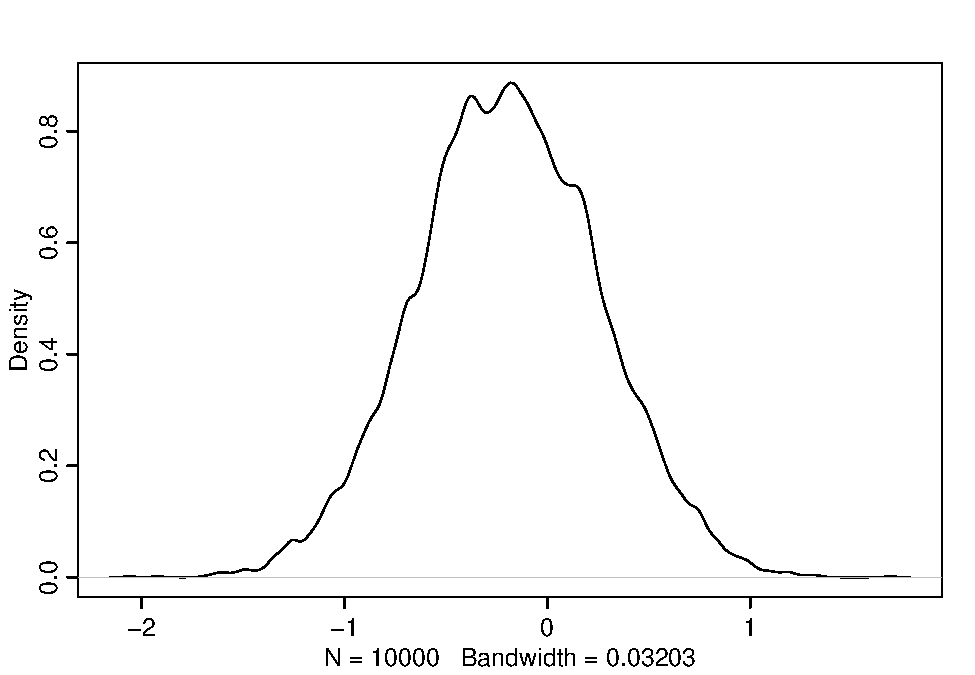
\includegraphics[width=20em]{ADM-Homework01_files/figure-latex/unnamed-chunk-1-1} \end{center}

\begin{center}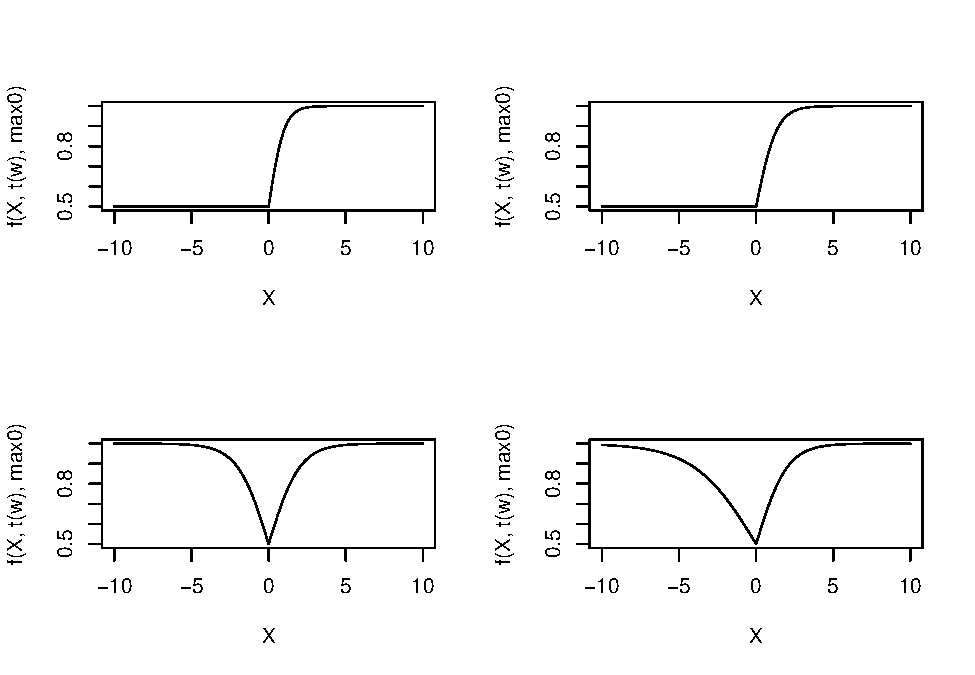
\includegraphics[width=20em]{ADM-Homework01_files/figure-latex/unnamed-chunk-1-2} \end{center}

\section{Problem 3: Gradient descent}\label{problem-3-gradient-descent}

\subsection{1.}\label{section-6}

The \(f(x)\) is plotted as follows,

\begin{Shaded}
\begin{Highlighting}[]
\NormalTok{f =}\StringTok{ }\ControlFlowTok{function}\NormalTok{(x)\{}\OperatorTok{-}\KeywordTok{dnorm}\NormalTok{(x, }\DecValTok{0}\NormalTok{, }\DecValTok{1}\NormalTok{) }\OperatorTok{+}\StringTok{ }\FloatTok{0.5} \OperatorTok{*}\StringTok{ }\KeywordTok{dnorm}\NormalTok{(x, }\DecValTok{1}\NormalTok{, }\FloatTok{0.5}\NormalTok{) }\OperatorTok{-}\StringTok{ }\FloatTok{0.4} \OperatorTok{*}\StringTok{ }\KeywordTok{dnorm}\NormalTok{(x, }\DecValTok{2}\NormalTok{, }\FloatTok{0.4}\NormalTok{)\}}
\NormalTok{x =}\StringTok{ }\KeywordTok{seq}\NormalTok{(}\OperatorTok{-}\DecValTok{2}\NormalTok{, }\DecValTok{4}\NormalTok{, }\DataTypeTok{length.out =} \DecValTok{500}\NormalTok{)}
\NormalTok{graph =}\StringTok{ }\KeywordTok{spline}\NormalTok{(x, }\KeywordTok{f}\NormalTok{(x), }\DataTypeTok{n =} \DecValTok{1000}\NormalTok{)}
\KeywordTok{plot}\NormalTok{(graph, }\DataTypeTok{type =} \StringTok{'l'}\NormalTok{, }\DataTypeTok{xlab =} \StringTok{'x'}\NormalTok{, }\DataTypeTok{ylab =} \StringTok{'f(x)'}\NormalTok{)}
\end{Highlighting}
\end{Shaded}

\begin{center}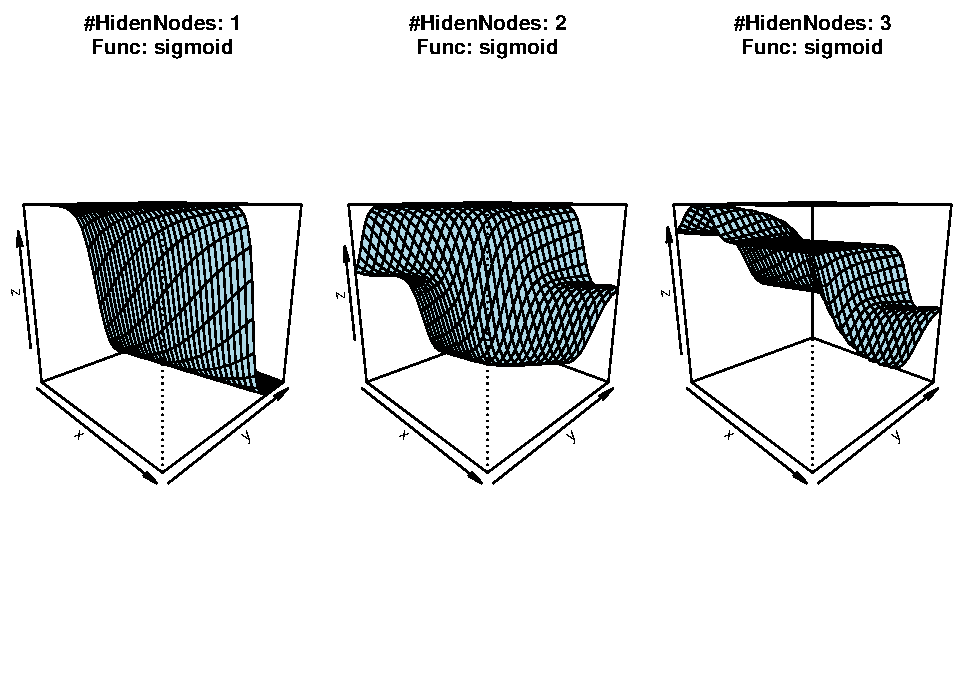
\includegraphics[width=30em]{ADM-Homework01_files/figure-latex/unnamed-chunk-2-1} \end{center}

\subsection{2.}\label{section-7}

\begin{Shaded}
\begin{Highlighting}[]
\NormalTok{f.prime =}\StringTok{ }\ControlFlowTok{function}\NormalTok{(x, }\DataTypeTok{delta =} \FloatTok{0.001}\NormalTok{)\{(}\KeywordTok{f}\NormalTok{(x }\OperatorTok{+}\StringTok{ }\NormalTok{delta) }\OperatorTok{-}\StringTok{ }\KeywordTok{f}\NormalTok{(x }\OperatorTok{-}\StringTok{ }\NormalTok{delta)) }\OperatorTok{/}\StringTok{ }\NormalTok{(}\DecValTok{2} \OperatorTok{*}\StringTok{ }\NormalTok{delta)\}}
\KeywordTok{print}\NormalTok{(}\KeywordTok{f.prime}\NormalTok{(}\OperatorTok{-}\DecValTok{2}\NormalTok{))}
\end{Highlighting}
\end{Shaded}

\begin{verbatim}
## [1] -0.1079819
\end{verbatim}

\subsection{3.}\label{section-8}

\begin{Shaded}
\begin{Highlighting}[]
\NormalTok{gred.des =}\StringTok{ }\ControlFlowTok{function}\NormalTok{(x1, }\DataTypeTok{epsilon =} \FloatTok{0.05}\NormalTok{)\{}
\NormalTok{    n =}\StringTok{ }\DecValTok{1}
\NormalTok{    x.data =}\StringTok{ }\KeywordTok{c}\NormalTok{(x1)}
    \ControlFlowTok{while}\NormalTok{(n }\OperatorTok{==}\StringTok{ }\DecValTok{1} \OperatorTok{||}\StringTok{ }\KeywordTok{abs}\NormalTok{(}\KeywordTok{f.prime}\NormalTok{(x1)) }\OperatorTok{>}\StringTok{ }\NormalTok{epsilon)\{}
\NormalTok{        pre =}\StringTok{ }\NormalTok{x1}
\NormalTok{        x1 =}\StringTok{ }\NormalTok{x1 }\OperatorTok{-}\StringTok{ }\KeywordTok{f.prime}\NormalTok{(x1) }\OperatorTok{/}\StringTok{ }\NormalTok{n}
\NormalTok{        x.data =}\StringTok{ }\KeywordTok{c}\NormalTok{(x.data, x1)}
\NormalTok{        n =}\StringTok{ }\NormalTok{n }\OperatorTok{+}\StringTok{ }\DecValTok{1}
\NormalTok{    \}}
    \KeywordTok{return}\NormalTok{(}\KeywordTok{list}\NormalTok{(n, x.data, x1, }\KeywordTok{f}\NormalTok{(x1)))}
\NormalTok{\}}
\end{Highlighting}
\end{Shaded}

When setting \(\epsilon = 0.05\) and \(\alpha_n = \frac{1}{n}\):

\begin{Shaded}
\begin{Highlighting}[]
\NormalTok{result =}\StringTok{ }\KeywordTok{gred.des}\NormalTok{(}\OperatorTok{-}\DecValTok{2}\NormalTok{, }\DataTypeTok{epsilon =} \FloatTok{0.05}\NormalTok{)}
\KeywordTok{print}\NormalTok{(result[}\DecValTok{1}\NormalTok{][[}\DecValTok{1}\NormalTok{]]) }\CommentTok{# Iteration times}
\end{Highlighting}
\end{Shaded}

\begin{verbatim}
## [1] 14945
\end{verbatim}

\begin{Shaded}
\begin{Highlighting}[]
\KeywordTok{print}\NormalTok{(}\KeywordTok{summary}\NormalTok{(result[}\DecValTok{2}\NormalTok{][[}\DecValTok{1}\NormalTok{]])) }\CommentTok{# All x_i}
\end{Highlighting}
\end{Shaded}

\begin{verbatim}
##    Min. 1st Qu.  Median    Mean 3rd Qu.    Max. 
## -2.0000 -0.4180 -0.3529 -0.4037 -0.3253 -0.3095
\end{verbatim}

\begin{Shaded}
\begin{Highlighting}[]
\KeywordTok{print}\NormalTok{(result[}\DecValTok{3}\NormalTok{][[}\DecValTok{1}\NormalTok{]]) }\CommentTok{# Final x_n}
\end{Highlighting}
\end{Shaded}

\begin{verbatim}
## [1] -0.3095104
\end{verbatim}

\begin{Shaded}
\begin{Highlighting}[]
\KeywordTok{print}\NormalTok{(result[}\DecValTok{4}\NormalTok{][[}\DecValTok{1}\NormalTok{]]) }\CommentTok{# Minimum of f(x)}
\end{Highlighting}
\end{Shaded}

\begin{verbatim}
## [1] -0.3673588
\end{verbatim}

\subsection{4.}\label{section-9}

\(x_1,\,...,x_{10}\) are plotted as follows,

\begin{center}\includegraphics[width=30em]{ADM-Homework01_files/figure-latex/unnamed-chunk-6-1} \end{center}

\subsection{5.}\label{section-10}

The hist graph is as follows,

\begin{center}\includegraphics[width=30em]{ADM-Homework01_files/figure-latex/unnamed-chunk-7-1} \end{center}

The minimum value of all 100 returns is as follows, which can be seen as
the global minimum of \(f(x)\).

\begin{verbatim}
## [1] -0.4009083
\end{verbatim}


\end{document}
